















\section*{ID: d3fe472f}
Triangle $A B C$ is similar to triangle $X Y Z$, such that $A, B$, and $C$ correspond to $X, Y$, and $Z$ respectively. The length of each side of triangle $X Y Z$ is 2 times the length of its corresponding side in triangle $A B C$. The measure of side $A B$ is 16 . What is the measure of side $X Y$ ?\\
A. 14\\
B. 16\\
C. 18\\
D. 32

\section*{ID: f9d40000}
In $\triangle X Y Z$, the measure of $\angle X$ is $23^{\circ}$ and the measure of $\angle Y$ is $66^{\circ}$. What is the measure of $\angle Z$ ?\\
A. $43^{\circ}$\\
B. $89^{\circ}$\\
C. $91^{\circ}$\\
D. $179^{\circ}$

\section*{ID: 0d3f51dc}
\begin{center}
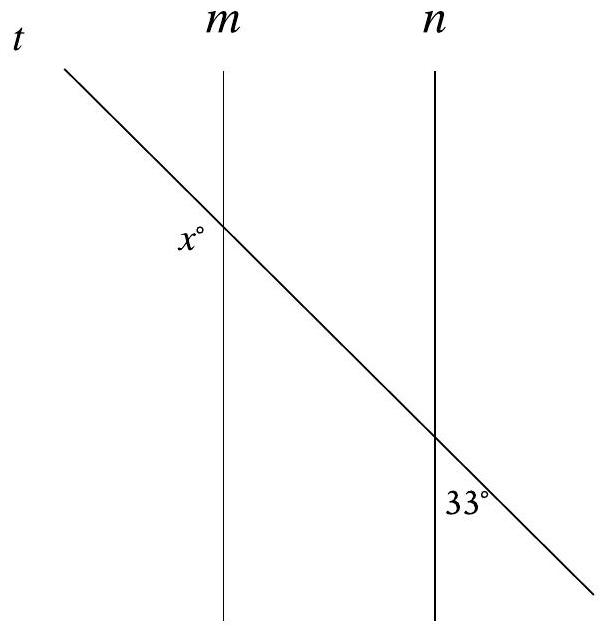
\includegraphics[max width=\textwidth]{2025_06_15_d0312806c0eedc278ae1g-23}
\end{center}

Note: Figure not drawn to scale.\\
In the figure, line $m$ is parallel to line $n$, and line $t$ intersects both lines. What is the value of $x$ ?\\
A. 33\\
B. 57\\
C. 123\\
D. 147

In triangle $J K L$, the measures of $\angle K$ and $\angle L$ are each $48^{\circ}$. What is the measure of $\angle J$, in degrees? (Disregard the degree symbol when entering your answer.)

\section*{ID: c7bed21d}
Quadrilateral $P^{\prime} Q^{\prime} R^{\prime} S^{\prime}$ is similar to quadrilateral $P Q R S$, where $P, Q, R$, and $S$ correspond to $P^{\prime}, Q^{\prime}, R^{\prime}$, and $S^{\prime}$, respectively. The measure of angle $P$ is $30^{\circ}$, the measure of angle $Q$ is $50^{\circ}$, and the measure of angle $R$ is $70^{\circ}$. The length of each side of $P^{\prime} Q^{\prime} R^{\prime} S^{\prime}$ is 3 times the length of each corresponding side of $P Q R S$. What is the measure of angle $P^{\prime}$ ?\\
A. $10^{\circ}$\\
B. $30^{\circ}$\\
C. $40^{\circ}$\\
D. $90^{\circ}$

At a certain time and day, the Washington Monument in Washington, DC, casts a shadow that is 300 feet long. At the same time, a nearby cherry tree casts a shadow that is 16 feet long. Given that the Washington Monument is approximately 555 feet tall, which of the following is closest to the height, in feet, of the cherry tree?\\
A. 10\\
B. 20\\
C. 30\\
D. 35

\section*{ID: dfc420b2}
\begin{center}
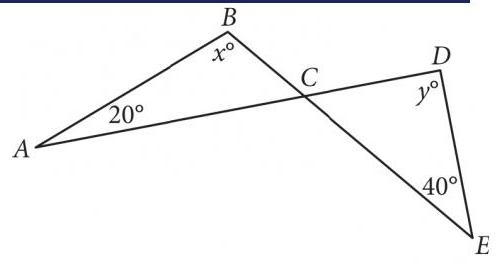
\includegraphics[max width=\textwidth]{2025_06_15_d0312806c0eedc278ae1g-27}
\end{center}

Note: Figure not drawn to scale.\\
In the figure above, $\overline{A D}$ intersects $\overline{B E}$ at $C$. If $x=100$, what is the value of $y$ ?\\
A. 100\\
B. 90\\
C. 80\\
D. 60

\section*{ID: 901e3285}
In triangle $A B C$, the measure of angle $A$ is $50^{\circ}$. If triangle $A B C$ is isosceles, which of the following is NOT a possible measure of angle $B$ ?\\
A. $50^{\circ}$\\
B. $65^{\circ}$\\
C. $80^{\circ}$\\
D. $100^{\circ}$\\
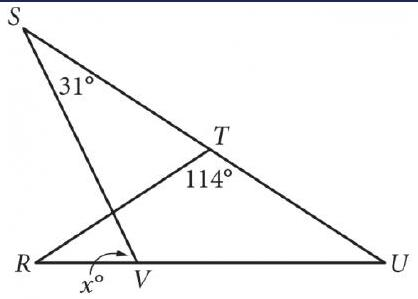
\includegraphics[max width=\textwidth, center]{2025_06_15_d0312806c0eedc278ae1g-29}

In the figure above, $R T=T U$.\\
What is the value of $x$ ?\\
A. 72\\
B. 66\\
C. 64\\
D. 58

\section*{ID: 2adbf1b1}
\begin{center}
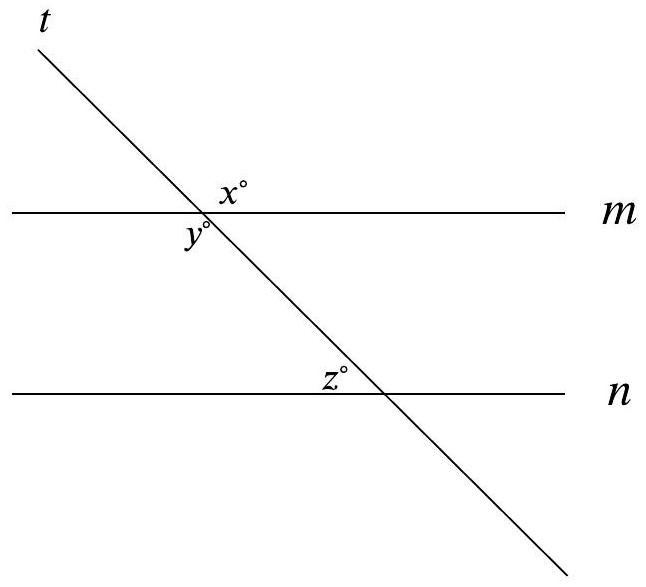
\includegraphics[max width=\textwidth]{2025_06_15_d0312806c0eedc278ae1g-30}
\end{center}

Note: Figure not drawn to scale.\\
In the figure, lines $m$ and $n$ are parallel. If $x=6 k+13$ and $y=8 k-29$, what is the value of $z ?$\\
A. 3\\
B. 21\\
C. 41\\
D. 139

ID: eeb4143c\\
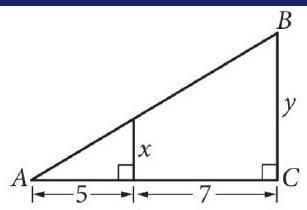
\includegraphics[max width=\textwidth, center]{2025_06_15_d0312806c0eedc278ae1g-31}

Note: Figure not drawn to scale.\\
The area of triangle $A B C$ above is at least 48 but no more than 60 . If $y$ is an integer, what is one possible value of $x$ ?

\section*{ID: 410bdbe6}
In the triangle above, $a=45$. What is the value of $b$ ?\\
A. 52\\
B. 59\\
C. 76\\
D. 104

\section*{ID: 087cdcfd}
\begin{center}
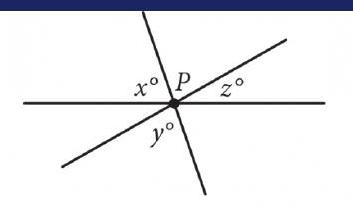
\includegraphics[max width=\textwidth]{2025_06_15_d0312806c0eedc278ae1g-33}
\end{center}

Note: Figure not drawn to scale.\\
In the figure, three lines intersect at point $P$. If $x=65$ and $y=75$, what is the value of $z$ ?\\
A. 140\\
B. 80\\
C. 40\\
D. 20

\section*{ID: afa3c48b}
\begin{center}
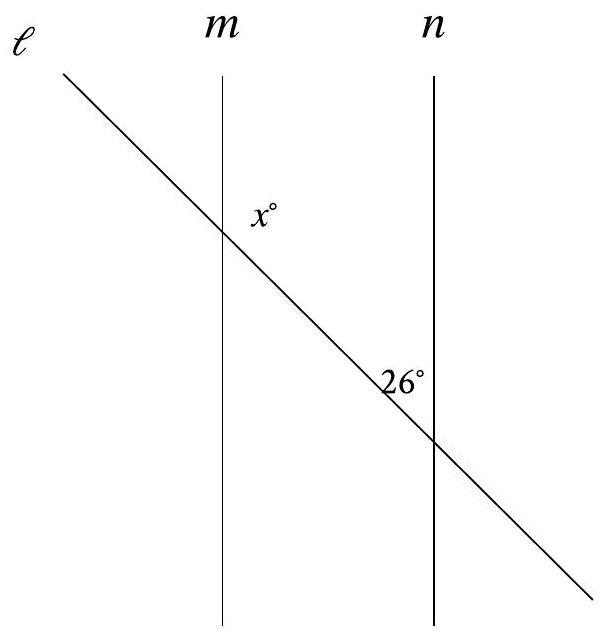
\includegraphics[max width=\textwidth]{2025_06_15_d0312806c0eedc278ae1g-34}
\end{center}

Note: Figure not drawn to scale.\\
In the figure shown, line $m$ is parallel to line $n$. What is the value of $x$ ?\\
A. 13\\
B. 26\\
C. 52\\
D. 154\\
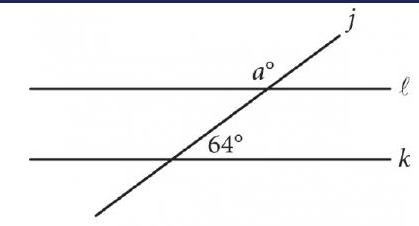
\includegraphics[max width=\textwidth, center]{2025_06_15_d0312806c0eedc278ae1g-35}

Note: Figure not drawn to scale.\\
In the figure above, lines $\ell$ and $k$ are parallel.\\
What is the value of $a$ ?\\
A. 26\\
B. 64\\
C. 116\\
D. 154

\section*{ID: f1747a6a}
In triangle $A B C$, the measure of angle $B$ is $52^{\circ}$ and the measure of angle $C$ is $17^{\circ}$. What is the measure of angle $A$ ?\\
A. $21^{\circ}$\\
B. $35^{\circ}$\\
C. $69^{\circ}$\\
D. $111^{\circ}$

\section*{ID: 1c3d613c}
\begin{center}
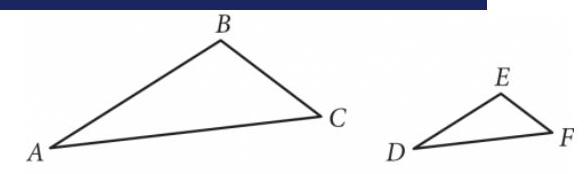
\includegraphics[max width=\textwidth]{2025_06_15_d0312806c0eedc278ae1g-37}
\end{center}

Note: Figures not drawn to scale.\\
Triangle $A B C$ and triangle $D E F$ are shown. The relationship between the side lengths of the two triangles is such that $\frac{A B}{D E}=\frac{B C}{E F}=\frac{A C}{D F}=3$. If the measure of angle $B A C$ is $20^{\circ}$, what is the measure, in degrees, of angle $E D F$ ? (Disregard the degree symbol when gridding your answer.)\\
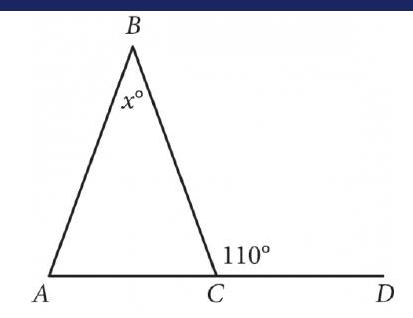
\includegraphics[max width=\textwidth, center]{2025_06_15_d0312806c0eedc278ae1g-38}

In the given figure, $\overline{A C}$ extends to point $D$. If the measure of $\angle B A C$ is equal to the measure of $\angle B C A$, what is the value of $x$ ?\\
A. 110\\
B. 70\\
C. 55\\
D. 40\\
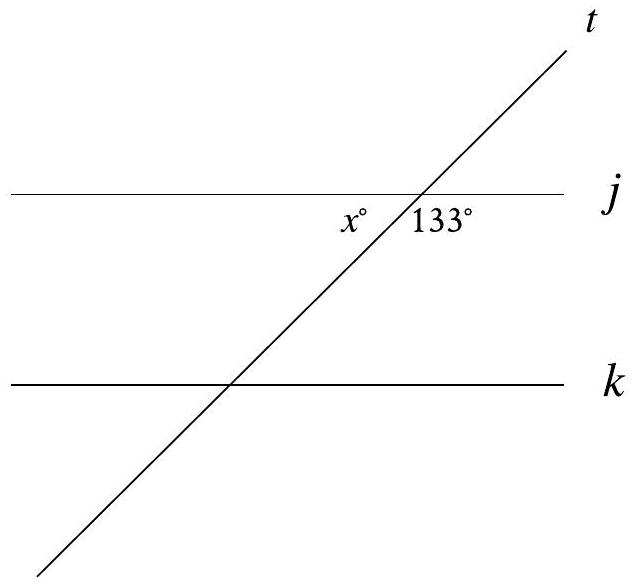
\includegraphics[max width=\textwidth, center]{2025_06_15_d0312806c0eedc278ae1g-39}

Note: Figure not drawn to scale.\\
In the figure, line $j$ is parallel to line $k$. What is the value of $x$ ?

In triangle $R S T$, angle $T$ is a right angle, point $L$ lies on $\overline{R S}$, point $K$ lies on $\overline{S T}$, and $\overline{L K}$ is parallel to $\overline{R T}$. If the length of $\overline{R T}$ is 72 units, the length of $\overline{L K}$ is 24 units, and the area of triangle $R S T$ is 792 square units, what is the length of $\overline{K T}$, in units?\\
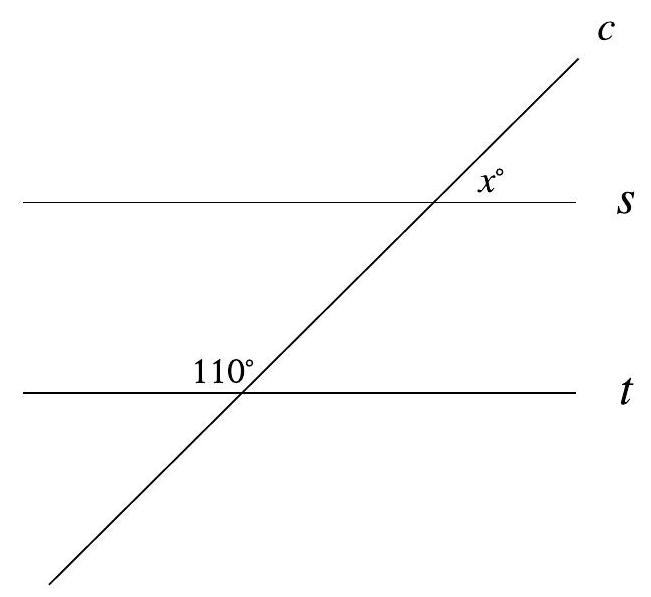
\includegraphics[max width=\textwidth, center]{2025_06_15_d0312806c0eedc278ae1g-41}

Note: Figure not drawn to scale.\\
In the figure shown, line $c$ intersects parallel lines $s$ and $t$. What is the value of $x$ ?

\section*{ID: 0bb39de4}
Triangles $A B C$ and $D E F$ are congruent, where $A$ corresponds to $D$, and $B$ and $E$ are right angles. The measure of angle $A$ is $18^{\circ}$. What is the measure of angle $F$ ?\\
A. $18^{\circ}$\\
B. $72^{\circ}$\\
C. $90^{\circ}$\\
D. $162^{\circ}$

\section*{ID: 6dd463ca}
Note: Figure not drawn to scale.\\
In the figure above, segments $A E$ and $B D$ are parallel. If angle $B D C$ measures $58^{\circ}$ and angle $A C E$ measures $62^{\circ}$, what is the measure of angle $C A E$ ?\\
A. $58^{\circ}$\\
B. $60^{\circ}$\\
C. $62^{\circ}$\\
D. $120^{\circ}$\\
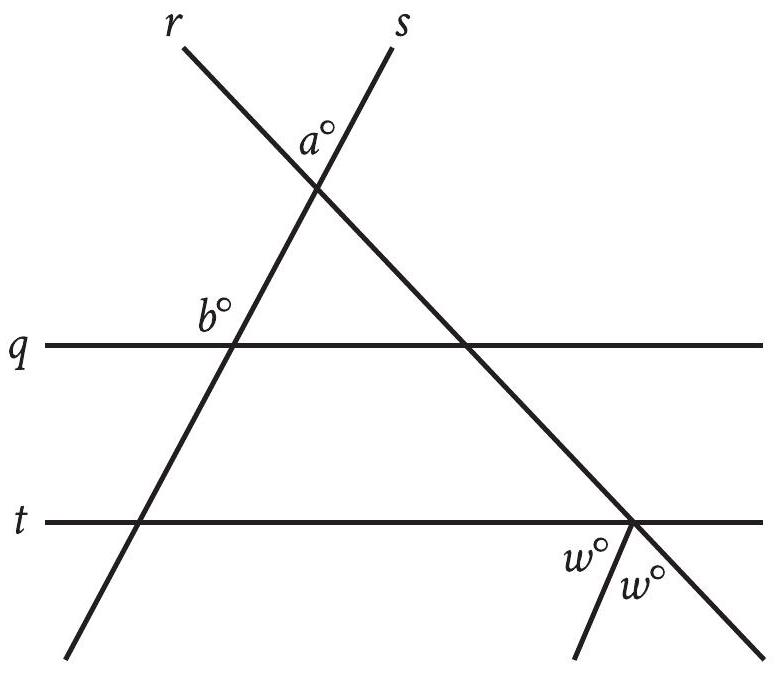
\includegraphics[max width=\textwidth, center]{2025_06_15_d0312806c0eedc278ae1g-44}

Note: Figure not drawn to scale.\\
In the figure, parallel lines $q$ and $t$ are intersected by lines $r$ and $s$. If $a=43$ and $b=122$, what is the value of $w$ ?

ID: 3828f53d\\
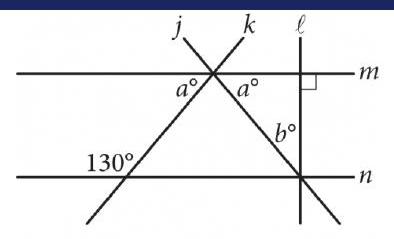
\includegraphics[max width=\textwidth, center]{2025_06_15_d0312806c0eedc278ae1g-45}

Note: Figure not drawn to scale.\\
In the figure above, lines $m$ and $n$ are parallel. What is the value of $b$ ?\\
A. 40\\
B. 50\\
C. 65\\
D. 80

\section*{ID: 4ff7b652}
Right triangles $L M N$ and $P Q R$ are similar, where $L$ and $M$ correspond to $P$ and $Q$, respectively. Angle $M$ has a measure of $53^{\circ}$. What is the measure of angle $Q$ ?\\
A. $37^{\circ}$\\
B. $53^{\circ}$\\
C. $127^{\circ}$\\
D. $143^{\circ}$

In a right triangle, the measure of one of the acute angles is $51^{\circ}$. What is the measure, in degrees, of the other acute angle?\\
A. 6\\
B. 39\\
C. 49\\
D. 51

\section*{ID: 36200a38}
\begin{center}
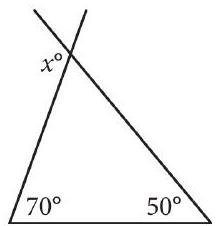
\includegraphics[max width=\textwidth]{2025_06_15_d0312806c0eedc278ae1g-48}
\end{center}

In the figure above, two sides of a triangle are extended. What is the value of $x$ ?\\
A. 110\\
B. 120\\
C. 130\\
D. 140

\section*{ID: 6a3fbec3}
\begin{center}
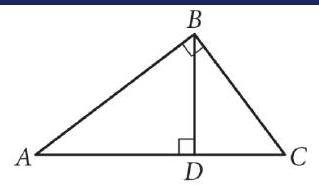
\includegraphics[max width=\textwidth]{2025_06_15_d0312806c0eedc278ae1g-49}
\end{center}

Note: Figure not drawn to scale.\\
In the figure above, $B D=6$ and $A D=8$.\\
What is the length of $\overline{D C}$ ?


